\section{Complete Registered Randomized Study}
\label{sec:supp-randomized-study}

This section preserves the detailed estimands, raw-realizability gates,
interaction diagnostics, sequential-prefix records, and frozen-pilot
comparison behind the randomized results summarized in the main paper.  The
study is a synthetic structural stress test of a fixed finite generator, not a
population sample or a population-frequency estimate.

\subsection{Synthetic estimands and exact fixture bridge}
\label{sec:supp-synthetic-estimands}

For fixture \(f\), horizon \(H\), and declared input set \(X_f\), define
\[
 \epsilon^{\rm proj}_{f,H}
 :=\max_{(b,L)\in X_f}
   |V_H^{\rm raw}(b,L)-V_H^K(b,\phi(L))|.
\]
For deletion \(L\to L^-\), frontier-only pruning \(L\to L^F\), and insertion,
the remaining exact-fixture estimands are
\[
\begin{gathered}
 \epsilon_F:=\lVert F_L-F_{L^-}\rVert_\infty,\quad
 \epsilon_C:=\mathbf 1\{C_L\ne C_{L^-}\},\quad
 \epsilon_V:=\max_b|V_H(b,L)-V_H(b,L^-)|,\\
 \operatorname{Loss}_H^F:=V_H(b,L)-V_H(b,L^F),\quad
 \lambda^F:=
 \frac{\operatorname{Loss}_H^F}{\beta^d\rho^d\pi C-\kappa},\quad
 \epsilon^{\rm dec}:=
 \Delta^{\rm tot}-\Delta^{\rm op}-\Delta^{\rm gen}.
\end{gathered}
\]
The ratio \(\lambda^F\) is used only when its denominator is positive.  For a
four-corner value fixture and a one-shot cost-covering set, define
\[
 J:=[V(F_1,C_1)-V(F_1,C_0)]-[V(F_0,C_1)-V(F_0,C_0)],
 \quad
 \mathcal R:=\{b:\Psi(b)-\kappa(b)\ge0\},
\]
and let \(c(\mathcal R)\) be the number of connected components on the ordered
belief grid.

The exact fixture outcomes are retained here as a bridge between those
estimands and the randomized design.
\begin{table}[htbp]
  \centering
  \small
  % Generated by julia/scripts/generate_manuscript_numerical_artifacts.jl.
% Sources: compression_experiments.csv and theorem_mechanism_{pruning_loss,decomposition,coverage_geometry}.csv.
\begin{tabular}{@{}p{0.22\linewidth}p{0.36\linewidth}p{0.34\linewidth}@{}}
\toprule
Mechanism & Registered exact input & Computed diagnostic \\
\midrule
Safe compression & Four-strategy, two-belief library & Minimum and greedy sizes both 3; frontier, closure, and value loss all zero \\
Frontier-only loss & Future rewards \(0,2,4,10,20,40\) & Loss \(R/2\) in all six cases; largest displayed loss 20 \\
Value decomposition & Operational-only, generative-only, and joint insertions & \((\Delta^{\op},\Delta^{\gen})=(3,0),(0,4),(3,1)\) \\
Monotone single gap & Potential \((0,1/2,3/2,3)\) & Upper-grid research set; one component \\
Single peak, bad kernel & Gap \((0,1,0)\), potential \((1,0,1)\) & Preservation assumption fails; two components \\
Separated multi-gap & Potential \((4,41/32,1/2,41/32,4)\) & Constant-cost research set has two components \\
\bottomrule
\end{tabular}

  \caption{Selected-instance outcomes from the exact mechanism fixtures.}
  \label{tab:supp-numerical-mechanisms}
\end{table}

The scaled frontier-only family obtains loss \(R/2\) at each
\(R\in\{0,2,4,10,20,40\}\).  The unit-cap fixture is the normalized result;
the bad-kernel and separated-gap fixtures retain their disconnection
diagnostics.

\subsection{Registered design and randomized estimands}
\label{sec:supp-randomized-estimands}

The randomized layer uses master seed
\texttt{6075990691714899803} and all \(N=1024\) registered horizon-four
trials.  The complete \(2^7\) factorial crosses sparse/dense frontiers,
low/high module overlap, weak/strong module complementarity, low/high project
cost, short/long duration, low/high admission, and low/high persistence.  Each
of the 128 cells has eight replicates.  The complete registry records 1,024
trial, catalog, project, and deletion seeds; all 4,096 are distinct.  The
initial design, sequential-precision amendment, and executable-protocol
amendment were locked before outcomes.

For trial \(t\), source library \(L_t\), pruning method \(m\), and pruned
library \(L_{tm}\), let
\[
 P_t(L):=\text{passive value},\qquad
 \Omega_t(L):=V_t(L)-P_t(L),
\]
\[
\begin{aligned}
 L^{\rm op}_{tm}&:=P_t(L_t)-P_t(L_{tm}),&
 L^{\rm gen}_{tm}&:=\Omega_t(L_t)-\Omega_t(L_{tm}),\\
 L^{\rm tot}_{tm}&:=V_t(L_t)-V_t(L_{tm})
                  =L^{\rm op}_{tm}+L^{\rm gen}_{tm},&
 r_{tm}&:=1-|L_{tm}|/|L_t|.
\end{aligned}
\]
For frontier-only pruning \(F\), define
\[
\begin{aligned}
 \widehat p_F&:=N^{-1}\sum_t\mathbf 1\{L^{\rm tot}_{tF}>0\},&
 \overline L_F^{+\mid+}
   &:=\frac{\sum_t[L^{\rm tot}_{tF}]_+}
            {\sum_t\mathbf 1\{L^{\rm tot}_{tF}>0\}},\\
 \widetilde L_F^{\max}
   &:=\max_t\frac{[L^{\rm tot}_{tF}]_+}{V_t(L_t)} .
\end{aligned}
\]
Strict positivity of every source value is a construction gate.  An
operationally silent generative asset \(s\in L_t\) satisfies
\[
 F_{L_t}=F_{L_t\setminus\{s\}},\qquad
 C_{L_t}\ne C_{L_t\setminus\{s\}},\qquad
 V_t(L_t)-V_t(L_t\setminus\{s\})>0 .
\]
Its asset-level frequency uses every noninactive source asset; a separate
library-level count records whether any such asset is present.

Every interaction observation starts from four actual raw libraries:
\[
\begin{array}{ll}
 L_{00}=L_{\rm base},&
 L_{10}=L_{\rm base}\cup A_F,\\
 L_{01}=L_{\rm base}\cup A_C,&
 L_{11}=L_{\rm base}\cup A_F\cup A_C,
\end{array}
\]
where \(A_F\) is closure-silent and frontier-improving, \(A_C\) is
frontier-silent and closure-improving, and the two additions commute.  All
four libraries use the same catalog and module closure.  Their frontiers,
closures, project laws, menus, transitions, and values are recomputed from raw
primitives.  With \(J_t\) defined by the four-corner difference above, the
sign frequencies are
\[
 \widehat p_{\rm sub}:=
 \frac{\#\{t:J_t<0\}}{1024},\qquad
 \widehat p_{\rm comp}:=
 \frac{\#\{t:J_t>0\}}{1024},
\]
with the analogous \(\widehat p_0\) for \(J_t=0\).  No synthetic compressed
rectangle enters these denominators.

All profiles, module rows, closure tables, kernels, project requirements,
admitted laws, raw updates, passive values, and Bellman values use
\texttt{Rational\{BigInt\}}.  Before writing any artifact, hard gates require
all 1,024 trials, all 4,096 raw corners, and every raw library to be valid;
every compressed state to have an enumerated raw witness; all raw/compressed
values to agree at every belief and remaining horizon \(0,\ldots,4\);
frontier-only passive loss to be zero; innovation-safe frontier, closure,
operational, generative, and total loss to be exactly zero; every signed
decomposition to close; and every displayed theorem-condition flag to be
computed from exact laws and action tables.  The completed audit records
47,458 raw-witness rows and 1,920 raw/compressed value comparisons per trial.

\subsection{Registered outcomes and factor slices}

\begin{table}[htbp]
  \centering
  \small
  \begin{tabular}{@{}p{0.48\linewidth}rr@{}}
    \toprule
    Registered estimand & Exact count & Exact estimate \\
    \midrule
    Positive frontier-only dynamic loss
      & \(398/1024\) & \(199/512\) \\
    Conditional mean positive loss
      & \(398\) positive trials & \(124909129/78249984\) \\
    Maximum normalized loss
      & \(1024\) trials & \(84963/222163\) \\
    Positive innovation-safe loss
      & \(0/1024\) & \(0\) \\
    Mean frontier-only compression ratio
      & \(1024\) trials & \(5/12\) \\
    Mean innovation-safe compression ratio
      & \(1024\) trials & \(1/8\) \\
    Silent generative asset
      & \(388/5120\) & \(97/1280\) \\
    Substitution, \(J_t<0\)
      & \(256/1024\) & \(1/4\) \\
    Complementarity, \(J_t>0\)
      & \(141/1024\) & \(141/1024\) \\
    Zero interaction, \(J_t=0\)
      & \(627/1024\) & \(627/1024\) \\
    \bottomrule
  \end{tabular}
  \caption{Registered finite-generator outcomes.  Ratios are structural
  stress-test frequencies, not estimates of real-population prevalence.}
  \label{tab:supp-randomized-library-v2}
\end{table}

Frontier-only pruning has positive loss in 398 trials; conditional on positive
loss, its mean magnitude is
\(124909129/78249984\approx1.5963\), and the largest normalized loss is
\(84963/222163\approx0.3824\).  Innovation-safe pruning has exact zero
frontier, closure, operational, generative, and total loss in every trial.
Its smaller mean compression ratio reflects the additional closure-
preservation constraint.  Silent generative carriers occur in 388 of 5,120
noninactive source-asset observations.

The primitive common-gap predicate is the mechanical conjunction of
frontier-independent project primitives and menus, poor-to-rich menu
inclusion, an antitone recursive descendant gap, nonnegative rich exposure,
zero poor exposure, and exact action-value identities.  It holds in 512
trials.  Those rows contain 255 substitutions, 257 zeros, and no
complementarity.  The other 512 rows are registered boundary constructions:
the 256 frontier-dependent-generator rows contain all 141 complementarities,
one substitution, and 114 zeros; the 256 positive-poor-exposure rows are all
zero.  Hence every positive \(J_t\) occurs where frontier-independent
generation and completion fail.  Marginally, complementarity is more frequent
under low cost than high cost (97 versus 44), short than long duration (107
versus 34), and high than low admission (95 versus 46).  These balanced factor
slices locate generated cases; they are neither causal comparisons nor a
theorem that complementarity is rare.

The companion exact interaction response preserves the registered 2,430-row
frontier--project boundary grid and five canonical four-corner fixtures:
primitive strict substitution, the saturation boundary, optimizer-switching
complementarity, frontier-dependent-success complementarity, and nonconstant
separability.  It crosses strict low/high frontier pairs, closure richness,
project cost, admission probability, descendant payoff, incumbent operating
reward, project duration, and frontier dependence of generator quality.  Each
row records the two closure increments, their cross difference, four selected
projects, four realizability flags, and the primitive sufficient-condition
certificate.  Nonrealizable rows remain diagnostic records but are never
aggregated into interaction-sign frequencies; Supplement~S2 reports the
corresponding interaction-theory interpretation.

\subsection{Sequential prefixes and descriptive uncertainty}

The sequential amendment fixed cumulative views at
\(N=50,100,200,300,500,750,1000,1024\) before outcomes and required the final
estimate to use all 1,024 trials.  The early prefixes are not claimed to be
factor-balanced.

\begin{table}[htbp]
\centering
\scriptsize
\setlength{\tabcolsep}{3pt}
\begin{tabular}{@{}rccccc@{}}
\toprule
\(N\) & Frontier loss & Safe loss & Silent asset &
Substitution & Complementarity\\
\midrule
50   & \(25/50\)   & \(0/50\)   & \(25/250\)   & \(27/50\)    & \(0/50\)\\
100  & \(45/100\)  & \(0/100\)  & \(45/500\)   & \(47/100\)   & \(0/100\)\\
200  & \(101/200\) & \(0/200\)  & \(101/1000\) & \(64/200\)   & \(39/200\)\\
300  & \(153/300\) & \(0/300\)  & \(153/1500\) & \(87/300\)   & \(69/300\)\\
500  & \(198/500\) & \(0/500\)  & \(192/2500\) & \(127/500\)  & \(69/500\)\\
750  & \(321/750\) & \(0/750\)  & \(315/3750\) & \(192/750\)  & \(130/750\)\\
1000 & \(396/1000\)& \(0/1000\) & \(388/5000\) & \(256/1000\) & \(141/1000\)\\
1024 & \(398/1024\)& \(0/1024\) & \(388/5120\) & \(256/1024\) & \(141/1024\)\\
\bottomrule
\end{tabular}
\caption{Cumulative registered event counts.  The silent-asset denominator is
five noninactive source assets per trial.  Prefixes diagnose simulation
precision and never select the final sample.}
\label{tab:supp-randomized-v2-stability-events}
\end{table}

At \(N=1024\), the descriptive Wilson intervals are
\([0.3593,0.4189]\) for frontier loss, \([0,0.00374]\) for innovation-safe
loss, \([0.06885,0.08335]\) for silent assets, \([0.2244,0.2774]\) for
substitution, and \([0.1179,0.1602]\) for complementarity.  The corresponding
Monte Carlo standard errors are \(0.08416\) for conditional mean positive
loss, \(0.00261\) for mean frontier compression, and \(0.00432\) for mean safe
compression.  Innovation-safe loss has zero events at every prefix and
therefore retains the registered sparse-event warning; complementarity has
zero events through \(N=100\), illustrating why the registered maximum cannot
be selected from an early sign.

\begin{table}[htbp]
\centering
\scriptsize
\setlength{\tabcolsep}{4pt}
\begin{tabular}{@{}rrrrr@{}}
\toprule
\(N\) & Positive support & Mean positive loss &
Frontier compression & Safe compression\\
\midrule
50   & 25  & \(1818477/1638400\)    & \(31/75\)     & \(9/100\)\\
100  & 45  & \(1623911/1474560\)    & \(5/12\)      & \(3/25\)\\
200  & 101 & \(5624367/3309568\)    & \(5/12\)      & \(51/400\)\\
300  & 153 & \(55259345/30081024\)  & \(187/450\)   & \(227/1800\)\\
500  & 198 & \(63735497/38928384\)  & \(1249/3000\) & \(47/375\)\\
750  & 321 & \(107121079/63111168\) & \(1873/4500\) & \(557/4500\)\\
1000 & 396 & \(124655857/77856768\) & \(5/12\)      & \(47/375\)\\
1024 & 398 & \(124909129/78249984\) & \(5/12\)      & \(1/8\)\\
\bottomrule
\end{tabular}
\caption{Cumulative mean diagnostics, all computed exactly.}
\label{tab:supp-randomized-v2-stability-means}
\end{table}

The complete 64-row cumulative table, 896-row factor-stratified table, exact
sample variances, interval values, warnings, and stabilization figure remain
in the registered artifacts indexed in Supplement~S7.

\subsection{Frozen pilot and policy-map diagnostics}

The earlier \(N=90\) study remains a frozen pilot and is not pooled with the
registered v2 estimates.  The two generators differ materially, so the
comparison below records provenance rather than a trend.

\begin{table}[htbp]
\centering
\scriptsize
\begin{tabular}{@{}
  p{0.34\linewidth}
  >{\centering\arraybackslash}p{0.25\linewidth}
  >{\centering\arraybackslash}p{0.31\linewidth}@{}}
\toprule
Quantity & Frozen pilot, \(N=90\) & Registered v2, \(N=1024\)\\
\midrule
Design & twelve marginally balanced three-level factors &
complete \(2^7\) factorial, eight replicates per cell\\
Positive frontier-only loss & \(8/90\) & \(398/1024\)\\
Conditional mean positive loss & \(3705/16384\) &
\(124909129/78249984\)\\
Mean frontier compression & \(22/45\) & \(5/12\)\\
Mean innovation-safe compression & \(2009/5400\) & \(1/8\)\\
Positive innovation-safe loss & \(0/90\) & \(0/1024\)\\
Silent generative assets & \(3/360\) & \(388/5120\)\\
Interaction comparison & omitted: no four-raw-witness gate &
\(256/141/627\) negative/positive/zero\\
\bottomrule
\end{tabular}
\caption{Frozen-pilot and v2 results are reported separately.  The pilot
interaction statistic is not compared because its synthetic compressed
rectangle did not require four raw witnesses.}
\label{tab:supp-randomized-pilot-comparison}
\end{table}

The separately locked resource extension reuses only the frozen v2 trial
registry and does not pool its outcomes with the parent study.  Every trial
enumerates all 32 inactive-containing sublibraries.  Complete optimizer
correspondences, capacity staircases, active pairwise breakpoints, price paths,
and channel arcs are indexed in Supplement~S7.

\begin{figure}[htbp]
  \centering
  % Generated by julia/scripts/generate_dynamic_policy_figure.jl.
% Source data: experiments/results/summaries/unified_comparative_statics_surface.csv.
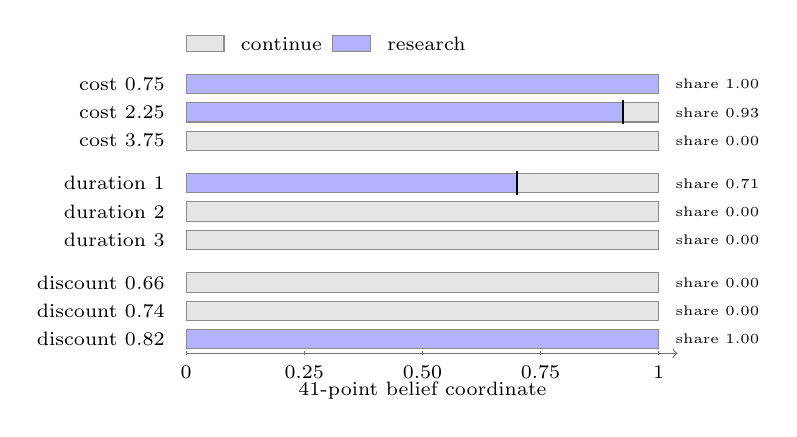
\begin{tikzpicture}[x=6.0cm,y=0.36cm,font=\scriptsize]
  \fill[black!10] (0,9.15) rectangle (0.08,9.7);
  \draw[black!45] (0,9.15) rectangle (0.08,9.7);
  \node[anchor=west] at (0.095,9.425) {continue};
  \fill[blue!30] (0.31,9.15) rectangle (0.39,9.7);
  \draw[black!45] (0.31,9.15) rectangle (0.39,9.7);
  \node[anchor=west] at (0.405,9.425) {research};
  \fill[blue!30] (0,7.66) rectangle (1,8.34);
  \draw[black!45] (0,7.66) rectangle (1,8.34);
  \node[anchor=east] at (-0.025,8.0) {cost \(0.75\)};
  \node[font=\tiny,anchor=west] at (1.015,8.0) {share 1.00};
  \fill[blue!30] (0,6.66) rectangle (0.925,7.34);
  \fill[black!10] (0.925,6.66) rectangle (1,7.34);
  \draw[black!45] (0,6.66) rectangle (1,7.34);
  \draw[black,line width=0.7pt] (0.925,6.58) -- (0.925,7.42);
  \node[anchor=east] at (-0.025,7.0) {cost \(2.25\)};
  \node[font=\tiny,anchor=west] at (1.015,7.0) {share 0.93};
  \fill[black!10] (0,5.66) rectangle (1,6.34);
  \draw[black!45] (0,5.66) rectangle (1,6.34);
  \node[anchor=east] at (-0.025,6.0) {cost \(3.75\)};
  \node[font=\tiny,anchor=west] at (1.015,6.0) {share 0.00};
  \fill[blue!30] (0,4.16) rectangle (0.7,4.84);
  \fill[black!10] (0.7,4.16) rectangle (1,4.84);
  \draw[black!45] (0,4.16) rectangle (1,4.84);
  \draw[black,line width=0.7pt] (0.7,4.08) -- (0.7,4.92);
  \node[anchor=east] at (-0.025,4.5) {duration \(1\)};
  \node[font=\tiny,anchor=west] at (1.015,4.5) {share 0.71};
  \fill[black!10] (0,3.16) rectangle (1,3.84);
  \draw[black!45] (0,3.16) rectangle (1,3.84);
  \node[anchor=east] at (-0.025,3.5) {duration \(2\)};
  \node[font=\tiny,anchor=west] at (1.015,3.5) {share 0.00};
  \fill[black!10] (0,2.16) rectangle (1,2.84);
  \draw[black!45] (0,2.16) rectangle (1,2.84);
  \node[anchor=east] at (-0.025,2.5) {duration \(3\)};
  \node[font=\tiny,anchor=west] at (1.015,2.5) {share 0.00};
  \fill[black!10] (0,0.66) rectangle (1,1.34);
  \draw[black!45] (0,0.66) rectangle (1,1.34);
  \node[anchor=east] at (-0.025,1.0) {discount \(0.66\)};
  \node[font=\tiny,anchor=west] at (1.015,1.0) {share 0.00};
  \fill[black!10] (0,-0.34) rectangle (1,0.34);
  \draw[black!45] (0,-0.34) rectangle (1,0.34);
  \node[anchor=east] at (-0.025,0.0) {discount \(0.74\)};
  \node[font=\tiny,anchor=west] at (1.015,0.0) {share 0.00};
  \fill[blue!30] (0,-1.34) rectangle (1,-0.66);
  \draw[black!45] (0,-1.34) rectangle (1,-0.66);
  \node[anchor=east] at (-0.025,-1.0) {discount \(0.82\)};
  \node[font=\tiny,anchor=west] at (1.015,-1.0) {share 1.00};
  \foreach \x/\label in {0/0,0.25/0.25,0.5/0.50,0.75/0.75,1/1} {
    \draw[black!55] (\x,-1.42) -- (\x,-1.57);
    \node[anchor=north] at (\x,-1.62) {\label};
  }
  \draw[black!55,->] (0,-1.5) -- (1.04,-1.5);
  \node[anchor=north] at (0.5,-2.18) {41-point belief coordinate};
\end{tikzpicture}

  \caption{Policy-map slices from the unified positive-duration response
  experiment.  The estimand in each row is the share of 41 enumerated belief
  points selecting research in a converged raw-derived Float64 solve; gray
  denotes Continue and blue denotes research.  Filled spans summarize the
  connected finite-grid action set and the boundary line is a grid cutoff,
  not a continuous root or smooth interpolation.  All duration rows are
  strictly positive, use \(P_B^d\), and apply the active-operation flag.}
  \label{fig:supp-dynamic-research-policy-regions}
\end{figure}

\clearpage
